\documentclass[main.tex,fontsize=8pt,paper=a4,paper=portrait,DIV=calc,]{scrartcl}
% Document
\usepackage[T1]{fontenc}
\usepackage[utf8]{inputenc}
\usepackage[dvipsnames]{xcolor}
\usepackage[nswissgerman,english]{babel} 
\usepackage{hyperref}
\renewcommand{\familydefault}{\sfdefault}

% Format
\usepackage[top=5mm,bottom=1mm,left=5mm,right=5mm]{geometry}
%\setlength{\headheight}{\baselineskip}
%\setlength{\headsep}{0mm}

%\usepackage{scrlayer-scrpage}
%\clearpairofpagestyles
%\chead{{\bfseries\TITLE, \AUTHOR, \pagename~\thepage}}

%\addtokomafont{pagehead}{\upshape}

\usepackage{multicol}
\setlength{\columnsep}{2mm}
\setlength{\columnseprule}{0.1pt}

% Math
\usepackage{amsmath}
\usepackage{amssymb}
\usepackage{amsfonts}

% Code
\usepackage{fancyvrb, etoolbox, listings, xcolor}
%\usemintedstyle{bw}

%\newminted[shell]{bash}{
%fontsize=\footnotesize,
%fontfamily=tt,
%breaklines=true,
%frame=single,
%framerule=0.1pt,
%framesep=2mm,
%tabsize=2
%}
%\newminted{css}{
%breaklines=true,
%tabsize=4,
%autogobble=true,
%escapeinside=||,
%stripall=true,
%stripnl=true,
%}

    \definecolor{lightgray}{rgb}{0.95, 0.95, 0.95}
    \definecolor{darkgray}{rgb}{0.4, 0.4, 0.4}
    \definecolor{purple}{rgb}{0.65, 0.12, 0.82}
    \definecolor{ocherCode}{rgb}{1, 0.5, 0} % #FF7F00 -> rgb(239, 169, 0)
    \definecolor{blueCode}{rgb}{0, 0, 0.93} % #0000EE -> rgb(0, 0, 238)
    \definecolor{greenCode}{rgb}{0, 0.6, 0} % #009900 -> rgb(0, 153, 0)
    \definecolor{teal}{rgb}{0.0, 0.5, 0.5}

\lstdefinestyle{code}{
    identifierstyle=\color{black},
    keywordstyle=\color{blue}\bfseries\small,
    ndkeywordstyle=\color{greenCode}\bfseries\small,
    stringstyle=\color{ocherCode}\ttfamily\small,
    commentstyle=\color{teal}\ttfamily\textit\small,
    basicstyle=\ttfamily\small,
    breakatwhitespace=false,         
    breaklines=true,                 
    captionpos=b,                    
    keepspaces=true,                 
    showspaces=false,                
    showstringspaces=false,
    showtabs=false,                  
    tabsize=2,
    belowskip=-5pt
}



% Images
\usepackage{graphicx}
\newcommand{\pic}{\includegraphics[scale=0.3]}
\graphicspath{{Screenshots/}{../Screenshots}}
\makeatletter
\def\pictext#1#2{%
    \@ifnextchar[{%
    \pictext@iiiii{#1}{#2}%
    }{%
      \pictext@iiiii{#1}{#2}[0.5,0.4,0.3]% Default is 5
    }%
}
\def\pictext@iiiii#1#2[#3,#4,#5]{\begin{minipage}{#3\textwidth}\includegraphics[scale=#4]{#1}\end{minipage}\begin{minipage}{#5\textwidth}#2\end{minipage}}
\def\minipg#1#2{%
    \@ifnextchar[{%
    \minipg@iiii{#1}{#2}%
    }{%
      \minipg@iiii{#1}{#2}[0.3,0.6]% Default is 5
    }%
}
\def\minipg@iiii#1#2[#3,#4]{\vspace{0.8mm}\begin{minipage}{#3\textwidth}#1\end{minipage}\begin{minipage}{#4\textwidth}#2\end{minipage}{\vspace{0.8mm}}}
\makeatother

%\newenvironment{minty}[2]% environment name
%{% begin code
%  \begin{minipage}{#1}
%  \begin{minted}{#2}
%}%
%{% end code
%  \end{minted}
%  \end{minipage}
%  \end{minty}\ignorespacesafterend
%} 

% Smaller Lists
\usepackage{enumitem}
\setlist[itemize,enumerate]{leftmargin=3mm, labelindent=0mm, labelwidth=1mm, labelsep=1mm, nosep}
\setlist[description]{leftmargin=0mm, nosep}
\setlength{\parindent}{0cm}

% Smaller Titles
\usepackage[explicit]{titlesec}

%% Color Boxes
\newcommand{\sectioncolor}[1]{\colorbox{black!60}{\parbox{0.989\linewidth}{\color{white}#1}}}
\newcommand{\subsectioncolor}[1]{\colorbox{black!50}{\parbox{0.989\linewidth}{\color{white}#1}}}
\newcommand{\subsubsectioncolor}[1]{\colorbox{black!40}{\parbox{0.989\linewidth}{\color{white}#1}}}
\newcommand{\paragraphcolor}[1]{\colorbox{black!30}{\parbox{0.989\linewidth}{\color{white}#1}}}
\newcommand{\subparagraphcolor}[1]{\colorbox{black!20}{\parbox{0.989\linewidth}{\color{white}#1}}}

%% Title Format
\titleformat{\section}{\vspace{0.5mm}\bfseries}{}{0mm}{\sectioncolor{\thesection~#1}}[{\vspace{0.5mm}}]
\titleformat{\subsection}{\vspace{0.5mm}\bfseries}{}{0mm}{\subsectioncolor{\thesubsection~#1}}[{\vspace{0.5mm}}]
\titleformat{\subsubsection}{\vspace{0.5mm}\bfseries}{}{0mm}{\subsubsectioncolor{\thesubsubsection~#1}}[{\vspace{0.5mm}}]
\titleformat{\paragraph}{\vspace{0.5mm}\bfseries}{}{0mm}{\paragraphcolor{\theparagraph~#1}}[{\vspace{0.5mm}}]
\titleformat{\subparagraph}{\vspace{0.5mm}\bfseries}{}{0mm}{\subparagraphcolor{\thesubparagraph~#1}}[{\vspace{0.5mm}}]

%% Title Spacing
\titlespacing{\section}{0mm}{0mm}{0mm}
\titlespacing{\subsection}{0mm}{0mm}{0mm}
\titlespacing{\subsubsection}{0mm}{0mm}{0mm}
\titlespacing{\paragraph}{0mm}{0mm}{0mm}
\titlespacing{\subparagraph}{0mm}{0mm}{0mm}

%% format cells
\usepackage[document]{ragged2e}
\usepackage{array, makecell}
\renewcommand{\arraystretch}{2}
\newcommand{\mc}{\makecell[{{m{1\linewidth}}}]}



\begin{document}
\tableofcontents

\lstset{
    language=Python,
    style=code,
}

\newcommand{\TITLE}{AI Applications}
\newcommand{\AUTHOR}{Fabio Lenherr}
\setcounter{tocdepth}{1}

\section{CNN Convolutional Neural Networks}

\subsection{Keras}
A python library that wraps tensorflow for classification.\newline
We will use this in this module to classify images like so:\newline
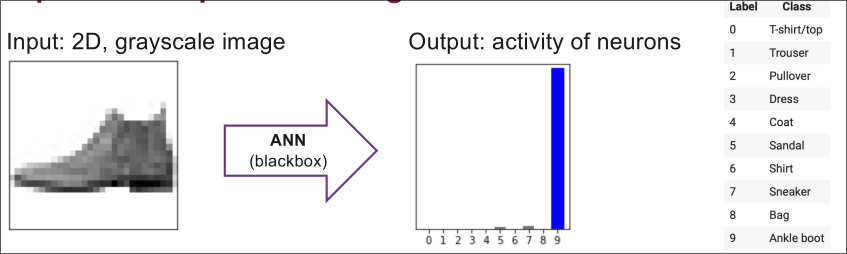
\includegraphics[scale=0.4]{2023_02_20_12_32_47.png}

\subsection{Flattening}
When we convert an image into a long vector, we lose information in the human sense, or rather make it hidden.\newline
todo, explain what is hidden and why


\section{Convolution}
\subsection{Firing of neurons}
Neurons are clearly connected to something very specific, this would then also be reflected in the artificial neural network. In other words, neuron 1 handles horizontal lines, another a line with a slight angle and so-on.\newline
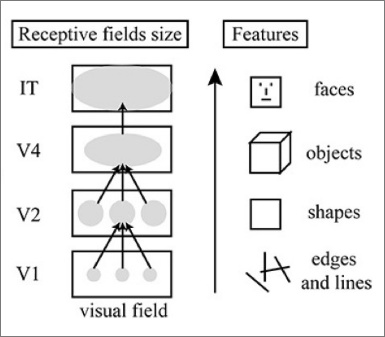
\includegraphics[scale=0.4]{2023_02_20_02_19_00.png}

\subsection{mathematical model of a feature detector}
\begin{itemize}
\item \textcolor{purple}{Two Inputs}\newline
  \begin{itemize}
  \item \textcolor{orange}{a picture}\newline
    Note that rgb would give you 3 channels red, green and blue
  \item \textcolor{orange}{A filter(kernel)}\newline
  \begin{itemize}
  \item  an m by n matrix in the simplest case (1 channel, grayscale).
  \item an m by n x 3 "stack of matrices" in the case of a 3 channel input (e.g. an RGB image)
  \item an m by n x d "stack of matrices". The depth of the kernel must equal the number of input channels.
  \end{itemize} 
\end{itemize} 
\item \textcolor{purple}{One Output}\newline
  A feature map (where is the thing that we wanted to search / determine by)\newline
  One convolution produces one feature map. Even if the input and the filter have multiple channels, the output of the convolution has one channel.
\item \textcolor{purple}{The Operation: Convolution}\newline
  We convolve the input image with the convolutional kernel
\end{itemize} 

\subsection{Example of convolution}
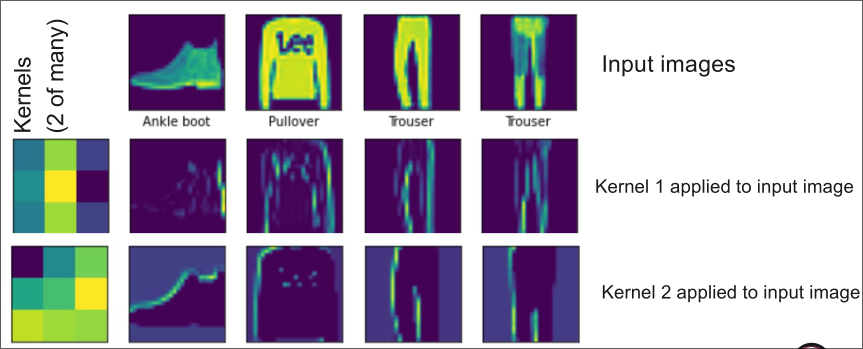
\includegraphics[scale=0.4]{2023_02_20_02_23_12.png}\newline
As you can see here, a filter will be used to detect something specific, like a pattern.\newline
\textcolor{purple}{This means that you will be combining multiple different filters in order to properly figure out what picture the underlying image is composed of.}\newline
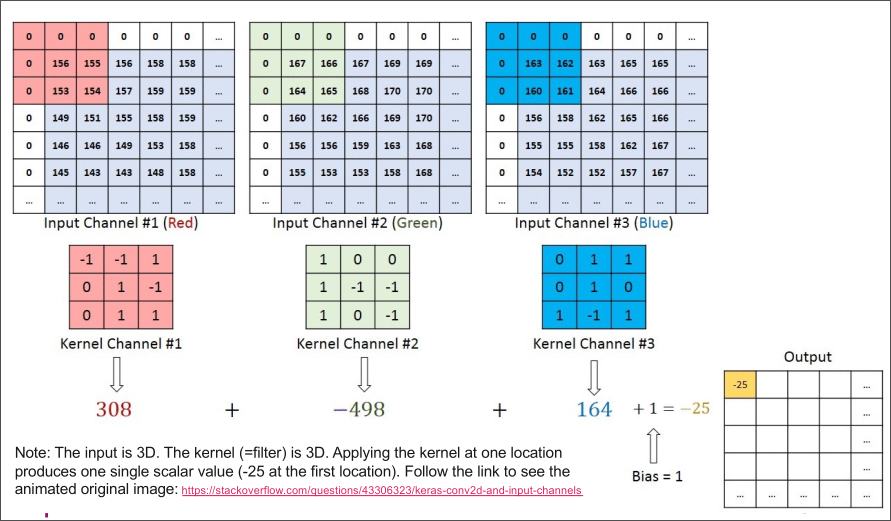
\includegraphics[scale=0.4]{2023_02_20_02_23_46.png}\newline
\textcolor{purple}{Explanation for the first calculation: 0 * -1 + 0 * -1 + 0 * 1 + 0 * 0 + 156 * 1 + 155 * -1 + 0 * 0 + 153 * 1 + 154 * 1 = 308}\newline
multiply each number in the top red square with the number in the same position in the bottom square.
We then proceed to do this for all channels (complexity of input, 3 for rgb), which \emph{will then be combined to 1 single output value}.\newline
This output value will then also be combined with a \emph{bias}.\newline
\textcolor{purple}{The entire reason we do this, is so that we can have an easier time calculating the images with a pc.}

\subsection{Reasons for convolution}
\begin{itemize}
\item \textcolor{purple}{Features can be detected independent of location -> filters will always find what they are supposed/created to find}
\item \textcolor{purple}{This calculation is done in parallel, which is very fast for gpus when doing matrix calculations! -> Hence the use of tensorflow with cuda!}
\item \textcolor{purple}{Shared weights mean using the same \emph{kernel values}, this reduces the use of a singular value for each neuron. -> more processing etc}
\end{itemize} 

\subsection{Stride}
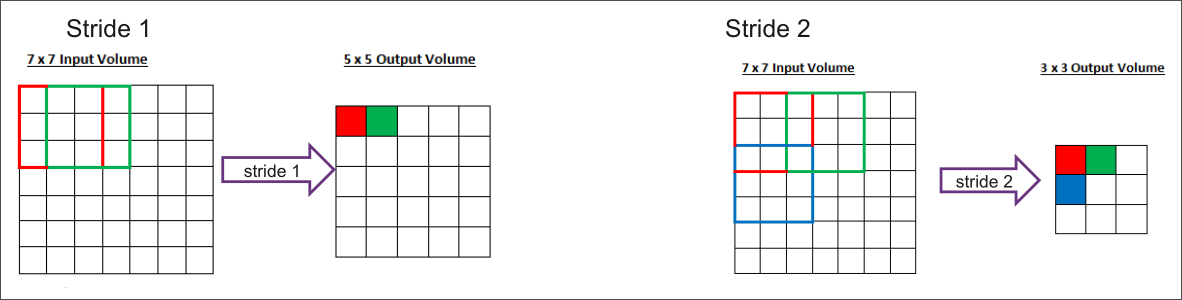
\includegraphics[scale=0.4]{2023_02_20_02_44_29.png}\newline
\textcolor{purple}{Stride is simply the offset by which we move towards the right and the bottom when we move to the next calculation.}\newline
The default value here is 1, which means Stride 1.

\subsection{Padding}
\minipg{
Padding is simply the edge of the matrix that has been predefined.\newline
A same padding is made entirely of 0's!
}{
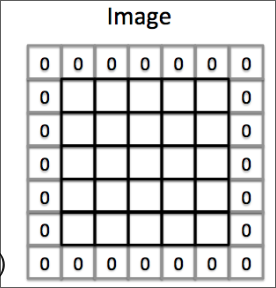
\includegraphics[scale=0.4]{2023_02_20_02_47_01.png}
}[0.45,0.4]

\subsection{Max Pooling}
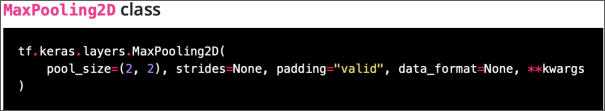
\includegraphics[scale=0.4]{2023_02_20_02_46_05.png}\newline
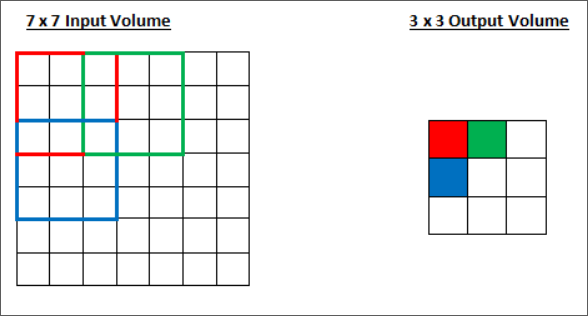
\includegraphics[scale=0.4]{2023_02_20_02_48_45.png}\newline
In this case we only take the \emph{max} value instead of some sum.\newline
This leaves you with rgb again instead of a mixed value!!

\subsection{Example with Keras}
\begin{lstlisting}
model = Sequential([
  layers.Rescaling(1./255, input_shape=(img_height, img_width, 3)),
  layers.Conv2D(16, 3, padding='same', activation='relu'),
  layers.MaxPooling2D(),
  layers.Conv2D(32, 3, padding='same', activation='relu'),
  layers.MaxPooling2D(),
  layers.Conv2D(64, 3, padding='same', activation='relu'),
  layers.MaxPooling2D(),
  layers.Flatten(),
  layers.Dense(128, activation='relu'),
  layers.Dense(num_classes)
])
\end{lstlisting}

\end{document}
